\begin{center}
	ĐỀ ÔN TẬP KIỂM TRA GIỮA HỌC KỲ I – MÔN VẬT LÝ 11\\
	Thời gian làm bài: 50 phút \\
	(Không kể thời gian phát đề)\\
\end{center}
\section{Trắc nghiệm \textit{(6,0 điểm)}}
\ANSMCQ{
	\begin{center}
		\begin{tabular}{|m{2.8em}|m{2.8em}|m{2.8em}|m{2.8em}|m{2.8em}|m{2.8em}|m{2.8em}|m{2.8em}|m{2.8em}|m{2.8em}|}
			\hline
			1D & 2A & 3C & 4A & 5B & 6D & 7A & 8A & 9C & 10A\\
			\hline
			11C & 12B & 13C & 14D & 15A & 16B & 17B & 18A & 19C & 20C\\
			\hline
		\end{tabular}
	\end{center}}

\begin{enumerate}[label=\bfseries Câu \arabic*:]
	\item Chuyển động của vật nào dưới đây không phải là dao động cơ?
	\begin{mcq}
		\item Chuyển động của pittong trong xilanh khi động cơ hoạt động.
		\item Chuyển động của con lắc đồng hồ gắn trong đồng hồ quả lắc.
		\item Chuyển động của chiếc lá nổi trên mặt nước khi có sóng truyền qua.
		\item Chuyển động của một vật trượt trên mặt phẳng nghiêng.
	\end{mcq}
\hideall{
\textbf{Đáp án D.}\\
Dao động cơ là sự chuyển động qua lại của một vật quanh vị trí cân bằng. Sự chuyển động của một vật trượt trên mặt phẳng nghiêng không phải là dao động cơ.
}

\item Biên độ dao động là 
\begin{mcq}
	\item độ dịch chuyển cực đại của vật tính từ vị trí cân bằng.
	\item độ dịch chuyển cực tiểu của vật tính từ vị trí cân bằng.
	\item độ dịch chuyển cực đại của vật tính từ vị trí biên.
	\item độ dịch chuyển cực tiểu của vật tính từ vị trí biên.
\end{mcq}
\hideall{
\textbf{Đáp án A.}
}

\item 
{Hình bên là đồ thị toạ độ theo thời gian của ba chuyển động. Chuyển động ứng với đồ thị nào là dao động điều hoà 
	\begin{center}
		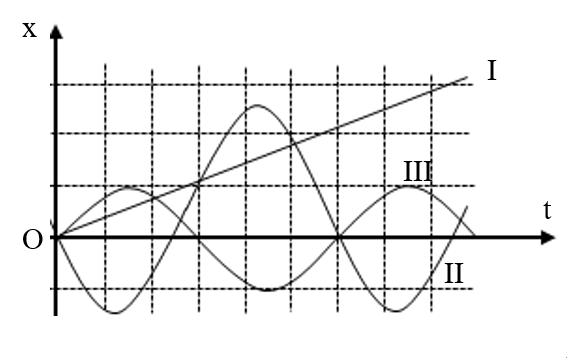
\includegraphics[width=0.4\linewidth]{../figs/D11-1-1}
\end{center}}
{\begin{mcq}(2)
		\item Đồ thị I.
		\item Đồ thị II.
		\item Đồ thị III.
		\item Đồ thị II và III.
\end{mcq}}
{\hideall{
		\textbf{Đáp án C.}
}}

\item Một vật nhỏ dao động điều hoà theo một trục cố định. Đồ thị li độ của vật theo thời gian có dạng 
\begin{mcq}(4)
	\item hình sin.	
	\item đường tròn.
	\item đường thẳng. 
	\item đường elip.
\end{mcq}
\hideall{
\textbf{Đáp án A.}
}

\item Công thức tính chu kì dao động của con lắc lò xo là
\begin{mcq}(4)
	\item $T=2\pi\sqrt{\dfrac{k}{m}}$.
	\item $T=2\pi\sqrt{\dfrac{m}{k}}$.
	\item $T=\dfrac{\pi}{2}\sqrt{\dfrac{m}{k}}$.
	\item $T=\sqrt{\dfrac{k}{m}}$.
\end{mcq}
\hideall{
\textbf{Đáp án B.}
}

\item Một vật nặng có khối lượng $m$, dao động điều hoà với phương trình $x=A\cos\omega t$. Cơ năng của vật là
\begin{mcq}(4)
	\item $m\omega A^2$.
	\item $\dfrac{1}{2}m\omega A^2$.
	\item $m\omega^2A^2$.
	\item $\dfrac{1}{2}m\omega^2A^2$.
\end{mcq}
\hideall{
\textbf{Đáp án D.}\\
Cơ năng của vật dao động điều hoà $W=\dfrac{1}{2}\omega^2A^2$.
}

\item Một con lắc đơn gồm vật nặng có khối lượng $m$, dây treo có chiều dài $\ell$ đang dao động tại nơi có gia tốc trọng trường $g$. Thế năng của con lắc ở li độ góc $\alpha$ là
\begin{mcq}(2)
	\item $W_t=mg\ell\left(1-\cos\alpha\right).$
	\item $W_t=mg\ell\left(1-\sin\alpha\right).$
	\item $W_t=mg\ell\cos\alpha.$
	\item $W_t=mg\ell\sin\alpha.$
\end{mcq}
\hideall{
\textbf{Đáp án A.}\\
}

\item Một vật dao động điều hòa đang chuyển động từ vị trí biên về vị trí cân bằng. Nhận xét nào sau đây là đúng?
\begin{mcq}
	\item Năng lượng của vật đang chuyển hóa từ thế năng sang động năng.
	\item Thế năng tăng dần và động năng giảm dần.
	\item Cơ năng của vật tăng dần đến giá trị lớn nhất.
	\item Thế năng của vật tăng dần nhưng cơ năng của vật không đổi.
\end{mcq}
\hideall{
\textbf{Đáp án A.}
}
\item Mỗi khi xe buýt đến bến, xe chỉ tạm dừng nên không tắt máy. Hành khách trên xe nhận thấy thân xe dao động, dao động này là
\begin{mcq}(2)
	\item dao động tắt dần.
	\item dao động duy trì.
	\item dao động cưỡng bức.
	\item dao động riêng.
\end{mcq}
\hideall{
\textbf{Đáp án C.}
}

\item Dao động tắt dần là dao động
\begin{mcq}(2)
\item có biên độ giảm dần theo thời gian. 
\item có chu kì giảm dần theo thời gian.
\item có động năng giảm dần theo thời gian.	
\item có tần số giảm dần theo thời gian.
\end{mcq}
\hideall{
\textbf{Đáp án A.}
}

\item Tác hại nào sau đây gây ra \textbf{không phải} do cộng hưởng?
\begin{mcq}
	\item Máy đầm hoạt động có thể gây ra rung lắc, nứt tường nhà.
	\item Động cơ ô tô hoạt động có thể gây rung lắc khung xe rất mạnh.
	\item Xe dao động mạnh khi qua “ổ gà” nên phải chế tạo bộ phận giảm xóc.
	\item Âm thanh quá lớn có thể làm chảy máu tai.
\end{mcq}
\hideall{
\textbf{Đáp án C.}
}

\item Một con lắc đơn dao động điều hoà thực hiện 10 dao động toàn phần trong thời gian $\SI{16}{\second}$. Biết gia tốc trọng trường $g=\xsi{\pi^2}{\meter/\second^2}$, chiều dài con lắc là
\begin{mcq}(4)
	\item $\SI{0.9}{\meter}$.
	\item $\SI{0.64}{\meter}$.
	\item $\SI{0.81}{\meter}$.
	\item $\SI{1.8}{\meter}$.
\end{mcq}
\hideall{
\textbf{Đáp án B.}\\
$$T=\dfrac{t}{N}=2\pi\sqrt{\dfrac{\ell}{g}}\Rightarrow \ell=\SI{0.64}{\meter}.$$
}

\item Một vật dao động điều hoà với phương trình $x=\xsi{4\cos\left(4\pi t-\dfrac{\pi}{4}\right)}{\centi\meter}$. Chu kì dao động của vật là
\begin{mcq}(4)
	\item $\xsi{4\pi}{\second}$.
	\item $\SI{2}{\second}$.
	\item $\SI{0.5}{\second}$.
	\item $\xsi{2\pi}{\second}$.
\end{mcq}
\hideall{
\textbf{Đáp án C.}
Chu kì dao động của vật:
$$T=\dfrac{2\pi}{\omega}=\SI{0.5}{\second}.$$
}

\item {Một vật dao động điều hoà có đồ thị li độ - thời gian được mô tả như hình bên. Gia tốc của vật dao động tại thời điểm $t=\SI{3}{\second}$ là
	\begin{center}
		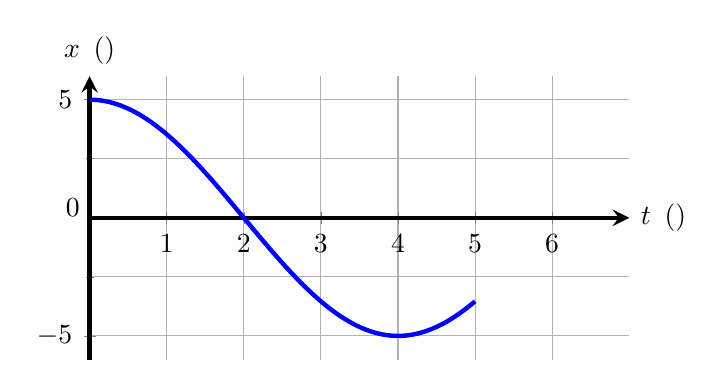
\begin{tikzpicture}  
			\begin{axis}[  ultra thick,
				xmin=0,  
				xmax=7,  
				xtick={0,1,...,6},
				ytick={-5,0,5},
				minor x tick num=0,
				minor y tick num=1,
				ymin=-6,  
				ymax=6, 
				y=0.3cm,
				samples=300,
				axis lines=center, 
				grid style={step=1, color=gray!60!white},
				grid=both,
				xlabel=$t\ \left(\si{\second}\right)$, 
				ylabel=$x\ \left(\si{\centi\meter}\right)$, 
				every axis y label/.style={at=(current axis.above origin),anchor=south},  
				every axis x label/.style={at=(current axis.right of origin),anchor=west},  ]
				\addplot [ultra thick, blue, smooth, domain=0:5] {5*cos(deg(pi*x/4))}; 
			\end{axis}  
			\node[label={[left]90:0}] at (0,1.8){};
		\end{tikzpicture}
	\end{center}
	
\begin{mcq}(4)
	\item $\SI{2.77}{\centi\meter/\second^2}$.
	\item $\SI{-2.18}{\centi\meter/\second^2}$.
	\item $\SI{-2.77}{\centi\meter/\second^2}$.
	\item $\SI{2.18}{\centi\meter/\second^2}$.
\end{mcq}}
\hideall{
\textbf{Đáp án D.}\\
Chu kì dao động của vật
$$T=\SI{8}{\second}\Rightarrow \omega=\dfrac{2\pi}{T}=\xsi{\dfrac{\pi}{4}}{\radian/\second}$$
Phương trình li độ của vật:
$$x=\xsi{5\cos\left(\dfrac{\pi}{4}t\right)}{\centi\meter}$$
Tại thời điểm $t=\SI{3}{\second}$ thì $x=\xsi{\dfrac{5\sqrt{2}}{2}}{\centi\meter}$.\\
Gia tốc của vật lúc này:
$$a=-\omega^2x=\SI{2.18}{\centi\meter/\second^2}.$$
}

\item Một vật dao động điều hoà có vận tốc cực đại là $v_\text{max}=\xsi{8\pi}{\centi\meter/\second}$ và gia tốc cực đại là $a_\text{max}=\xsi{16\pi^2}{\centi\meter/\second^2}$. Tần số góc của dao động là
\begin{mcq}(4)
	\item $\xsi{2\pi}{\radian/\second}$.
	\item $\xsi{4\pi}{\radian/\second}$.
	\item $\xsi{2\pi^2}{\radian/\second}$.
	\item $\xsi{4\pi^2}{\radian/\second}$.
\end{mcq}
\hideall{
\textbf{Đáp án A.}\\
Ta có:
\begin{align*}
	\begin{cases}
		a_\text{max}=\omega^2A\\
		v_\text{max}=\omega A
	\end{cases}
\Rightarrow \omega=\dfrac{a_\text{max}}{v_\text{max}}=\xsi{2\pi}{\radian/\second}
\end{align*}
}

\item Một vật dao động điều hoà với biên độ $A$ và cơ năng $W$. Mốc thế năng của vật ở vị trí cân bằng. Khi vật đi qua vị trí có li độ $\dfrac{2}{3}A$ thì động năng của vật là
\begin{mcq}(4)
	\item $\dfrac{7}{9}W$.
	\item $\dfrac{5}{9}W$.
	\item $\dfrac{4}{9}W$.
	\item $\dfrac{2}{9}W$.
\end{mcq}
\hideall{
	\textbf{Đáp án B.}\\
	Khi vật qua vị trí $x=\dfrac{2}{3}A$ thì 
$$\dfrac{W_t}{W}=\dfrac{x^2}{A^2}=\dfrac{4}{9}\Rightarrow W_t=\dfrac{4}{9}W\Rightarrow W_\text{đ}=W-W_\text{t}=\dfrac{5}{9}W.$$
}


\item 
{Đồ thị biểu diễn li độ theo thời gian của một vật dao động điều hoà được mô tả như hình bên. Pha ban đầu của dao động là
\begin{center}
	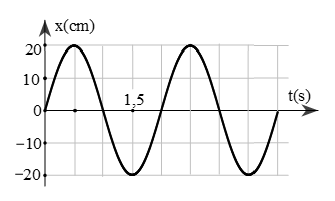
\includegraphics[width=0.4\linewidth]{../figs/D11-1-2}
\end{center}}
{\begin{mcq}(4)
	\item $\xsi{\dfrac{\pi}{2}}{\radian}$.
	\item $\xsi{-\dfrac{\pi}{2}}{\radian}$.
	\item $\xsi{\pi}{\radian}$.
	\item $\xsi{-\pi}{\radian}$.
	\end{mcq}}
{\hideall{
		\textbf{Đáp án B.}
	}}

\item Một chất điểm dao động điều hoà với phương trình vận tốc $v=\xsi{2\sqrt{2}\cos\left(2t+\dfrac{5\pi}{6}\right)}{\centi\meter/\second}$. Tại thời điểm vật có vận tốc tức thời $\SI{2}{\centi\meter/\second}$ thì li độ của vật có thể là
\begin{mcq}(4)
	\item $\SI{1}{\centi\meter}$.
	\item $\xsi{\sqrt{2}}{\centi\meter}$.
	\item $\SI{2}{\centi\meter}$.
	\item $\xsi{2\sqrt{2}}{\centi\meter}$.
\end{mcq}
\hideall{
\textbf{Đáp án A.}\\
Biên độ dao động:
$$A=\dfrac{v_\text{max}}{\omega}=\xsi{\sqrt{2}}{\centi\meter}$$
Áp dụng hệ thức độc lập thời gian:
$$\left(\dfrac{v}{v_\text{max}}\right)^2+\left(\dfrac{x}{A}\right)^2=1\Rightarrow x^2=A^2\left[1-\left(\dfrac{v}{v_\text{max}}\right)^2\right]=\pm\SI{1}{\centi\meter}.$$
}

\item 
{Cho một chất điểm dao động điều hoà quanh vị trí cân bằng O. Li độ biến thiên theo thời gian như mô tả trong đồ thị hình bên. Kẻ đường tiếp tuyến với đồ thị li độ ở thời điểm $t=\SI{0.75}{\second}$ thì thấy nó cắt trục $Ot$ ở giá trị $\SI{0.43}{\second}$. Vận tốc của chất điểm ở thời điểm đó gần với giá trị nào sau đây nhất?
\begin{center}
	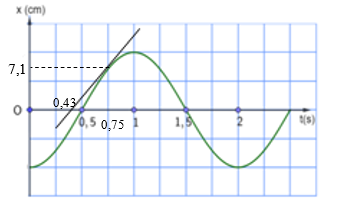
\includegraphics[width=0.4\linewidth]{../figs/D11-1-3}
\end{center}
\begin{mcq}(4)
	\item $\SI{8.1}{\centi\meter/\second}.$
	\item $\SI{-8.1}{\centi\meter/\second}.$
	\item $\SI{22.2}{\centi\meter/\second}.$
	\item $\SI{-22.2}{\centi\meter/\second}.$
\end{mcq}
}
{
\hideall{
\textbf{Đáp án C.}\\
Vận tốc tức thời của vật tại một thời điểm được xác định bằng độ dốc tiếp tuyến đồ thị $x-t$:
$$v=\tan\alpha=\dfrac{\Delta x}{\Delta t}=\dfrac{\SI{7.1}{\centi\meter}-\SI{0}{\centi\meter}}{\SI{0.75}{\second}-\SI{0.43}{\second}}\approx\SI{22.19}{\centi\meter/\second}.$$
}
}

\item 
{Chất điểm khối lượng $\SI{200}{\gram}$ dao động điều hoà quanh vị trí cân bằng O. Li độ của chất điểm biến thiên theo thời gian như đồ thị hình bên. Cơ năng của chất điểm trong quá trình dao động là
	\begin{center}
		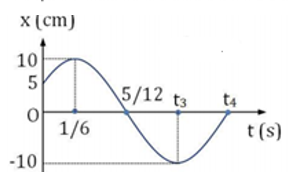
\includegraphics[width=0.35\linewidth]{../figs/D11-1-4}
	\end{center}
\begin{mcq}(4)
	\item $\SI{0.1}{\joule}$.
	\item $\SI{0.05}{\joule}$.
	\item $\SI{0.04}{\joule}$.
	\item $\SI{0.01}{\joule}$.
\end{mcq}
}
\hideall{
\textbf{Đáp án C.}\\
Biên độ dao động của chất điểm $A=\SI{10}{\centi\meter}=\SI{0.1}{\meter}$.
Chu kì dao động của chất điểm:
$$\dfrac{T}{4}=\xsi{\dfrac{5}{12}}{\second}-\xsi{\dfrac{1}{6}}{\second}=\xsi{0.25}{\second}\Rightarrow T=\SI{1}{\second}$$
Cơ năng của chất điểm trong quá trình dao động:
$$W=\dfrac{1}{2}m\omega^2A^2=\dfrac{1}{2}\cdot\left(\SI{0.2}{\kilogram}\right)\cdot\left(\dfrac{2\pi}{\SI{1}{\second}}\right)^2\cdot\left(\SI{0.1}{\meter}\right)^2\approx\SI{0.04}{\joule}.$$

}
\end{enumerate}
\section{Tự luận \textit{(4,0 điểm)}}
\begin{enumerate}[label=\bfseries Bài \arabic*:]
	\item Xét một con lắc lò xo đang dao động điều hoà với đồ thị gia tốc - thời gian như hình bên. Với lò xo được sử dụng có độ cứng $k=\SI{500}{\newton/\meter}$ và lấy $\pi^2=10$. Hãy xác định:
	\begin{center}
		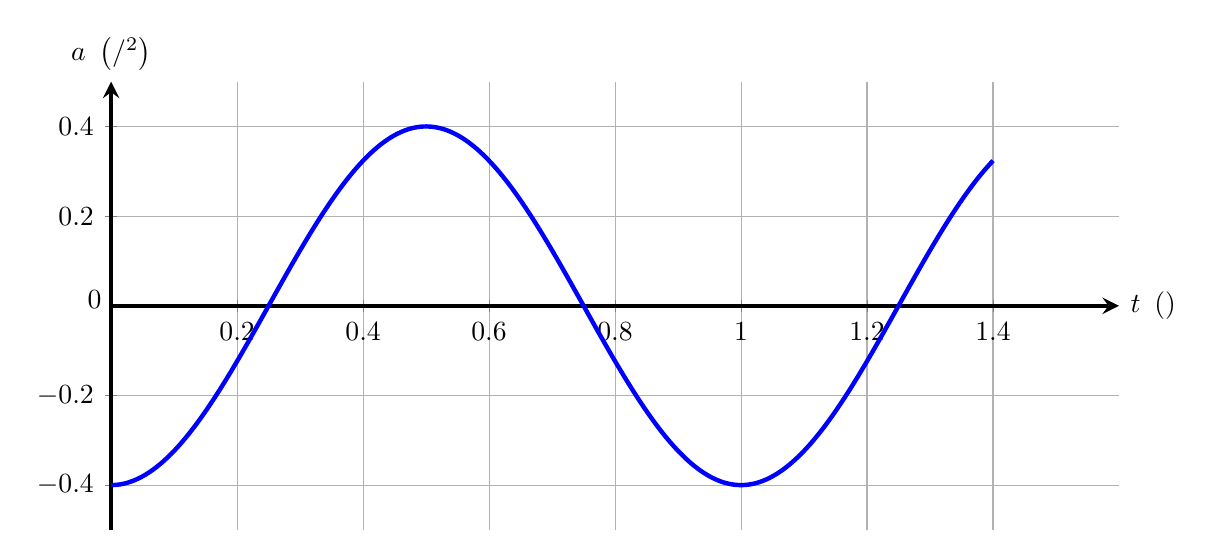
\begin{tikzpicture}  
			\begin{axis}[  ultra thick,
				xmin=0,  
				xmax=1.6,  
				xtick={0,0.2,...,1.4},
				ytick={-0.4,-0.2,...,0.4},
				minor x tick num=0,
				minor y tick num=0,
				ymin=-0.5,  
				ymax=0.5, 
				x=8cm,
				samples=300,
				axis lines=center, 
				grid style={step=0, color=gray!60!white},
				grid=both,
				xlabel=$t\ \left(\si{\second}\right)$, 
				ylabel=$a\ \left(\si{\meter/\second^2}\right)$, 
				every axis y label/.style={at=(current axis.above origin),anchor=south},  
				every axis x label/.style={at=(current axis.right of origin),anchor=west},  ]
				\addplot [ultra thick, blue, smooth, domain=0:1.4] {0.4*cos(deg(pi*x*2+pi))}; 
			\end{axis}  
			\node[label={[left]90:0}] at (0,2.8){};
		\end{tikzpicture}
	\end{center}
	\begin{enumerate}[label=\alph*)]
		\item Khối lượng của vật nặng.
		\item Li độ của vật tại thời điểm $t=\SI{1.4}{\second}$.
	\end{enumerate}
\hideall{
\begin{enumerate}[label=\alph*)]
	\item Dựa vào đồ thị, ta có: $T=\SI{1}{\second}\Rightarrow \omega=\dfrac{2\pi}{T}=\xsi{2\pi}{\radian/\second}$.\\
	Khối lượng của vật nặng:
	$$m=\dfrac{k}{\omega^2}=\dfrac{\SI{500}{\newton/\meter}}{\left(\xsi{2\pi}{\radian/\second}\right)^2}=\SI{12.5}{\kilogram}.$$
	\item Dựa vào đồ thị, ta có:
	$$a_\text{max}=\SI{0.4}{\meter/\second^2}\Rightarrow A=\dfrac{a_\text{max}}{\omega^2}=\dfrac{\SI{0.4}{\meter/\second^2}}{\left(\xsi{2\pi}{\radian/\second}\right)^2}=\SI{0.01}{\meter}=\SI{1}{\centi\meter}.$$
	Tại thời điểm ban đầu, gia tốc có giá trị cực tiểu nên vật ở vị trí biên dương, suy ra pha ban đầu của dao động là $\SI{0}{\radian}$.\\
	Phương trình li độ của vật dao động: 
	$$x=\xsi{\cos\left(2\pi t\right)}{\centi\meter}$$
	Li độ của vật tại thời điểm $t=\SI{1.4}{\second}$ là:
	$$x=\cos\left[\left(\xsi{2\pi}{\radian/\second}\right)\cdot\left(\SI{1.4}{\second}\right)\right]\approx\SI{-0.84}{\centi\meter}.$$
\end{enumerate}
}

\item Cho một dao động tắt dần, nếu xem gần đúng dao động tắt dần này là dao động điều hoà, cứ sau mỗi chu kì thì cơ năng của hệ sẽ giảm $\SI{24}{\percent}$. Hỏi sau khoảng bao nhiêu chu kì, biên độ của dao động sẽ giảm còn một nửa?
\hideall{
Cơ năng ban đầu của dao động 
$$W=\dfrac{1}{2}m\omega^2A^2$$
Cơ năng của dao động sau mỗi chu kì còn lại là $W'=0,76W$. Do đó, biên độ của dao động sau mỗi chu kì là $A_1=\sqrt{0,76}A_0$.\\
Vậy sau $N$ chu kì thì biên độ dao động còn lại là $A_N=\left(\sqrt{0,76}\right)^NA_0$.\\
Khi $A_N=\dfrac{1}{2}A_0$, ta thu được $N\approx5$.\\
Vậy sau khoảng 5 chu kì dao động thì biên độ dao động giảm còn 1 nửa.
}
\end{enumerate}